%!TEX program = pdflatex
\RequirePackage[l2tabu, orthodox]{nag}
\documentclass{book}
% 9 LaTeX packages everyone should use
\usepackage{amsmath}
\usepackage[a4paper]{geometry}
\usepackage{graphicx}
\usepackage{microtype}
\usepackage{siunitx}
\usepackage{booktabs}
\usepackage[colorlinks=false, pdfborder={0 0 0}]{hyperref}
\usepackage{cleveref}

\usepackage[scaled=0.92]{helvet}    % set Helvetica as the sans-serif font
\renewcommand{\rmdefault}{ptm}      % set Times as the default text font
% The following loads mtpro and defines some common MTPro options [2, 4]
\usepackage[subscriptcorrection,slantedGreek,nofontinfo]{mtpro2}

\usepackage[Lenny]{fncychap}


\begin{document}
\chapter{Distribution}
\section{$\chi^{2}$ distribution}

Let $z_{1},z_{2},\ldots,z_{k}$ be independent random variables with $z_{i}\sim \mathcal{N}(0,1)$ (iid), then
\begin{equation}
Z=z_{1}^{2}+z_{2}^{2}+\cdots+z_{k}^{2}=\sum_{i=1}^{n} z_{i} \sim \chi^{2}_{k}
\end{equation}

 $\chi^{2}$ is a class of distribution indexed by its degree of freedom, like the $t$-distribution. In fact, $\chi^{2}$ has a relation with $t$.

If $x_1 ,x_2,\ldots,x_n$ are independent random variables with $x_{i}\sim \mathcal{N}(\mu,\sigma)$, then
\begin{equation}
X =\sum_{i=1}^{n}\bigg(\frac{x_{i}-\mu}{\sigma}\bigg)^{2}\sim \chi^{2}_{n}
\end{equation}

Let $X_{1} \sim \chi^{2}_{n}$ and $X_{2} \sim \chi^{2}_{m}$. If $X_{1}$ and $X_{2}$ are independent, then
\begin{equation}
X_{1}+X_{2} \sim \chi^{2}_{n+m}.
\end{equation}

\begin{figure}[!htbp]
\centering
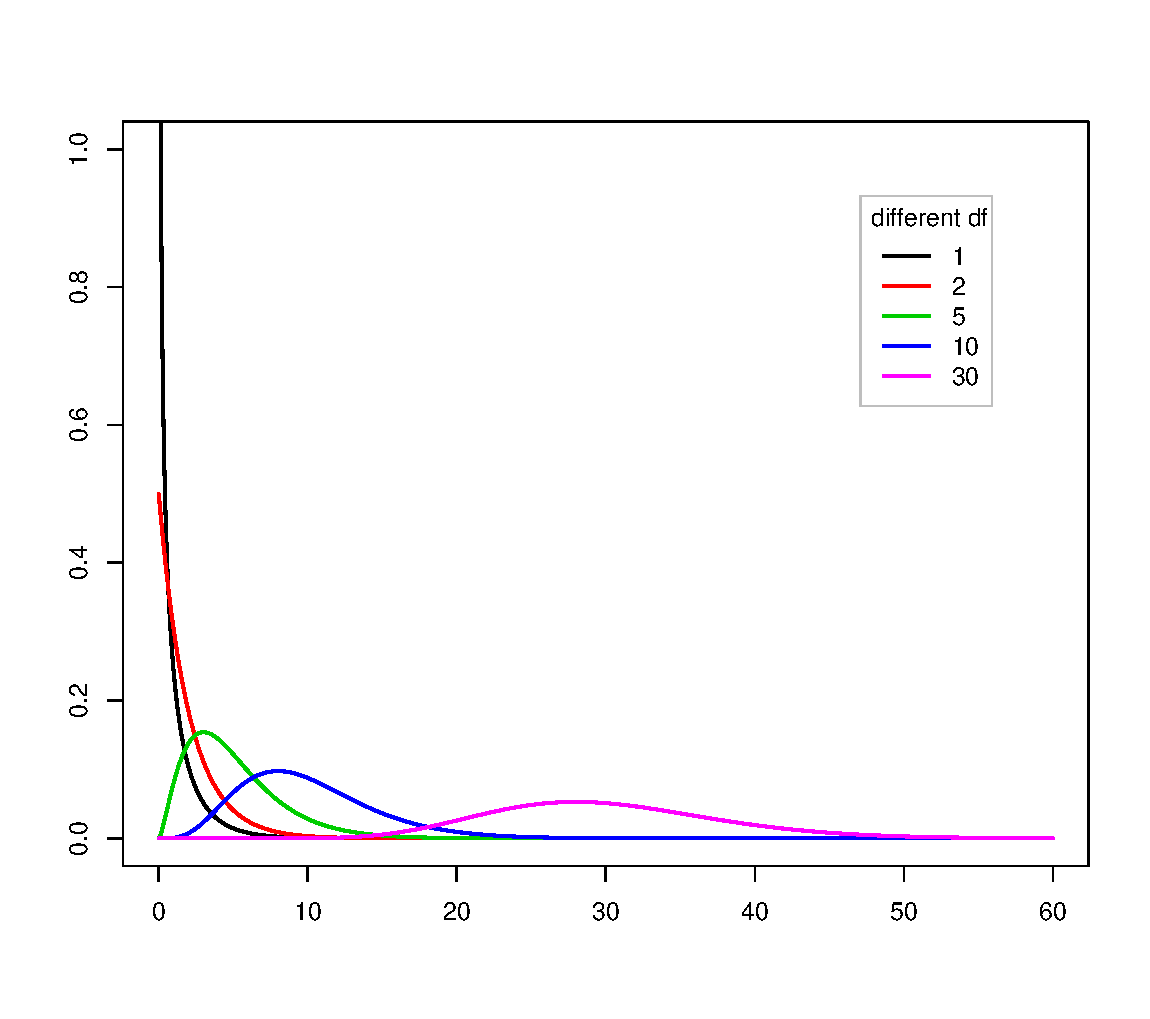
\includegraphics[width=0.6\textwidth]{./graph/chisq.pdf}
\caption{$\chi^{2}$ with different df}\label{fig:/graph/chisq.pdf}
\end{figure}






\end{document}
